%%%%%%%%%%%%%%%%%%%%%%%%%%%%%%%%%%%%%%%%%
% Beamer Presentation
% LaTeX Template
% Version 1.0 (10/11/12)
%
% This template has been downloaded from:
% http://www.LaTeXTemplates.com
%
% License:
% CC BY-NC-SA 3.0 (http://creativecommons.org/licenses/by-nc-sa/3.0/)
%
%%%%%%%%%%%%%%%%%%%%%%%%%%%%%%%%%%%%%%%%%

%----------------------------------------------------------------------------------------
%	PACKAGES AND THEMES
%----------------------------------------------------------------------------------------

\documentclass[czech]{beamer}

\mode<presentation> {

% The Beamer class comes with a number of default slide themes
% which change the colors and layouts of slides. Below this is a list
% of all the themes, uncomment each in turn to see what they look like.

%\usetheme{default}
%\usetheme{AnnArbor}
%\usetheme{Antibes}
%\usetheme{Bergen}
%\usetheme{Berkeley}
%\usetheme{Berlin}
%\usetheme{Boadilla}
%% \usetheme{CambridgeUS}
%\usetheme{Copenhagen}
%\usetheme{Darmstadt}
%\usetheme{Dresden}
%\usetheme{Frankfurt}
%\usetheme{Goettingen}
%\usetheme{Hannover}
%\usetheme{Ilmenau}
%\usetheme{JuanLesPins}
%\usetheme{Luebeck}
\usetheme{Madrid}
%\usetheme{Malmoe}
%\usetheme{Marburg}
%\usetheme{Montpellier}
%\usetheme{PaloAlto}
%\usetheme{Pittsburgh}
%\usetheme{Rochester}
%\usetheme{Singapore}
%\usetheme{Szeged}
%\usetheme{Warsaw}

% Change color to KMZ Brno I color
\definecolor{beamer@blendedblue}{RGB}{5,89,37}

% As well as themes, the Beamer class has a number of color themes
% for any slide theme. Uncomment each of these in turn to see how it
% changes the colors of your current slide theme.
%\usecolortheme{albatross}
%\usecolortheme{beaver}
%\usecolortheme{beetle}
%\usecolortheme{crane}
%\usecolortheme{dolphin}
%\usecolortheme{dove}
%\usecolortheme{fly}
%\usecolortheme{lily}
%\usecolortheme{orchid}
%\usecolortheme{rose}
%\usecolortheme{seagull}
%\usecolortheme{seahorse}
%\usecolortheme{whale}
%\usecolortheme{wolverine}

%\setbeamertemplate{footline} % To remove the footer line in all slides uncomment this line
%\setbeamertemplate{footline}[page number] % To replace the footer line in all slides with a simple slide count uncomment this line

%\setbeamertemplate{navigation symbols}{} % To remove the navigation symbols from the bottom of all slides uncomment this line
}

\beamertemplatenavigationsymbolsempty

\usepackage[czech]{babel}
\usepackage[utf8]{inputenc}
\usepackage[T1]{fontenc}
\usepackage{lmodern}
\usepackage{graphicx} % Allows including images
\usepackage{booktabs} % Allows the use of \toprule, \midrule and \bottomrule in tables
\usepackage{hyperref}

\deftranslation[to=Czech]{Example}{Příklad}

%----------------------------------------------------------------------------------------
%	TITLE PAGE
%----------------------------------------------------------------------------------------

\title[hJOP]{\normalsize hJOP\\\Large Chybové stavy a jejich řešení} % The short title appears at the bottom of every slide, the full title is only on the title page

\author{Jan Horáček} % Your name
\institute[KMŽ Brno I] % Your institution as it will appear on the bottom of every slide, may be shorthand to save space
{
Klub modelářů železnic Brno I \\ % Your institution for the title page
\medskip
\textit{jan.horacek@kmz-brno.cz} % Your email address
}
\date{24. února 2017} % Date, can be changed to a custom date

\begin{document}

\begin{frame}
\titlepage % Print the title page as the first slide
\end{frame}

%----------------------------------------------------------------------------------------
%	PRESENTATION SLIDES
%----------------------------------------------------------------------------------------

%------------------------------------------------
\section{Úvod}
%------------------------------------------------

\begin{frame}
\frametitle{Motivace}
\begin{itemize}
\item Zpříjemnit obsluhu.
\item Naučit obsluhu elegantně řešit neobvyklé situace.
	\begin{enumerate}
	\item Nezklouznout do ještě podivnějšího stavu.
	\item S co nejmenším dopadem na zbytek provozu a obsluhy (ideální stav =
	vedlejší stanice se o problému ani nedozví).
	\item Co nejrychleji.
	\end{enumerate}
\end{itemize}
\end{frame}

%------------------------------------------------

\begin{frame}
\frametitle{Jak na to?}
\begin{enumerate}
\item Pochopit základní vnitřní principy hJOP.
\item Popsat typické problémy.
	\begin{itemize}
	\item Zaměříme se na problémy, které vedou k zabránění stavění jízdní cesty.
	\end{itemize}
\item Vyzkoušet si vše prakticky.

\pause
~\\

\begin{block}{Co dnes dělat nebudeme}
Nebudeme interagovat přímo se serverem. Proč?
\end{block}

\end{enumerate}
\end{frame}

%------------------------------------------------

\begin{frame}
\frametitle{Zjednodušená logika hJOPserveru}
\begin{figure}
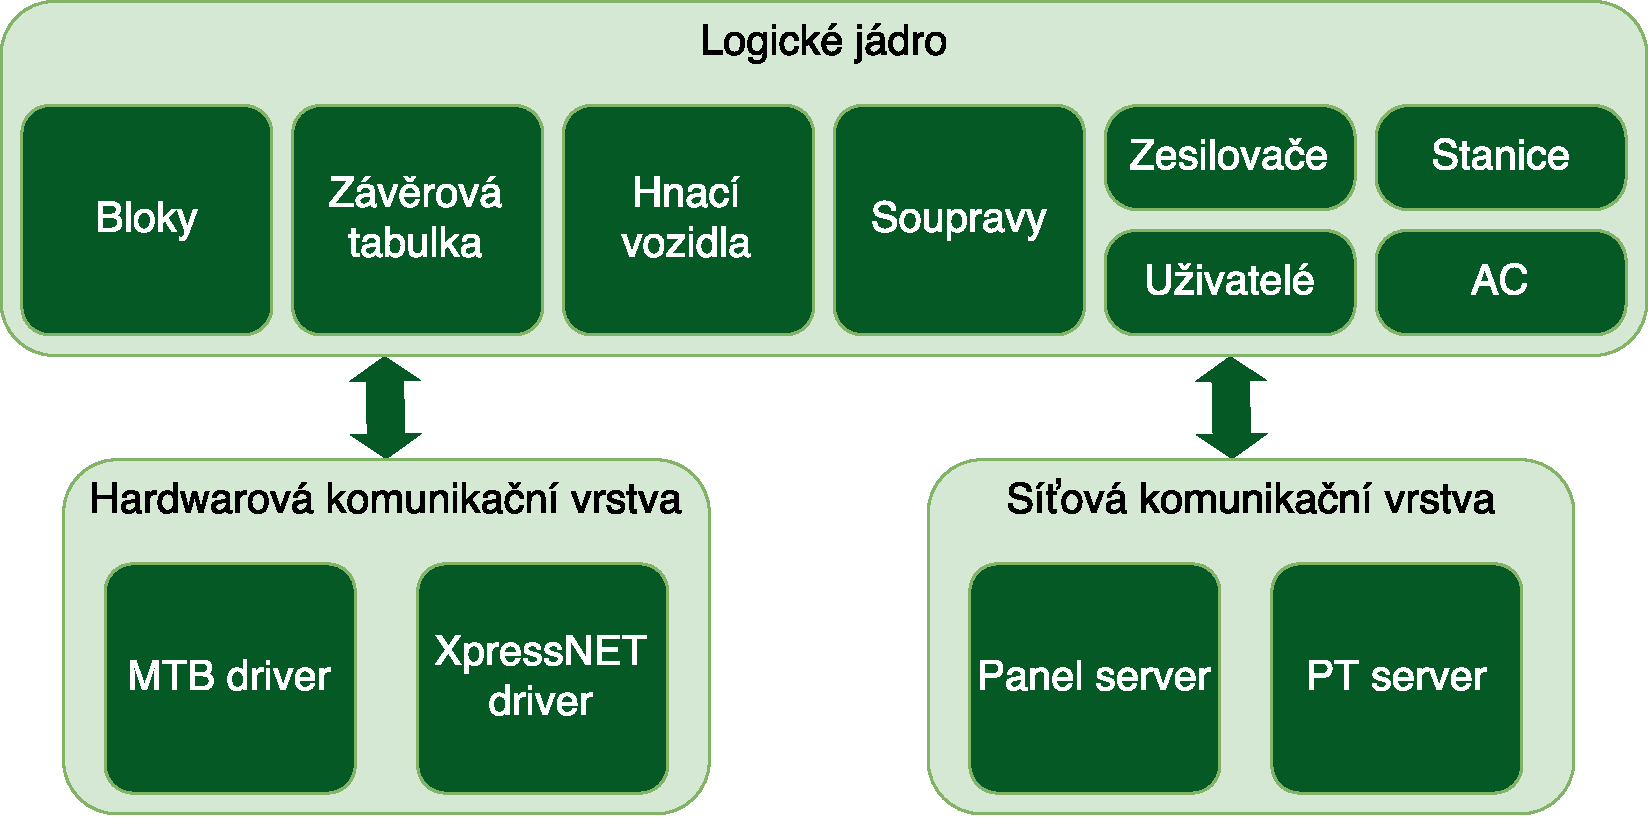
\includegraphics[width=\linewidth]{hJOPserver-log-scheme.pdf}
\end{figure}
\end{frame}

%------------------------------------------------
\section{Bloky}
%------------------------------------------------

\begin{frame}
\frametitle{Bloky}
\begin{itemize}
\item Server si udržuje databázi bloků.
\item Bloků je více typů: výhybka, úsek, infračidlo, návěstidlo, ...
\item Některé bloky mohou být vyvedeny na jeden či více (!) panelů.
\item \textbf{Název bloku lze zobrazit v panelu otevřením menu bloku}
(najet myší na blok $\rightarrow$ F2).
\end{itemize}
\end{frame}

%------------------------------------------------
\section{Jízdní cesty}
%------------------------------------------------

\begin{frame}
\frametitle{Jízdní cesty}
\begin{itemize}
\item hJOP si udržuje jízdní cesty pomocí editorem definované tabulky.
\item Seznam jízdních cest se někdy označuje pojmem \textit{závěrová tabulka}.
\item Jízdní cesty definuje editor při editaci, při provozu je tabulka prakticky
	neměnná, ačkoliv možnost změny tu je.
\end{itemize}
\end{frame}

%------------------------------------------------

\begin{frame}
\frametitle{Jízdní cesta}
Jízdní cesta je obecný pojem zahrnující tyto typy cest:
\begin{enumerate}
\item vlaková cesta,
\item posunová cesta,
\item nouzová vlaková cesta,
\item nouzová posunová cesta.
\end{enumerate}

~\\

hJOP dovoluje definovat vlakové a posunové cesty. Nouzové cesty se pak odvíjí
od příslušných vlakových a posunových cest dle závěrové tabulky.

\end{frame}

%------------------------------------------------

\begin{frame}
\frametitle{Záznam jízdní cesty}

Záznam jízdní cesty obsahuje tato data:

\begin{enumerate}
\begin{columns}[c]
\column{.45\textwidth}
\item název
\item id (číslo)
\item id bloku návěstidla
\item typ (vlaková, posunová)
\item návaznost na další návěstidlo
\item seznam id výhybek
\item seznam id úseků
\item seznam id odvratů
\item seznam id příslušenství
\item seznam id přejezdů

\column{.45\textwidth}
\item dodatečné podmínky
	\begin{itemize}
	\item na zámek
	\item (na polohu výhybky)
	\end{itemize}
\item variantní body
\item návaznost na trať
\item rychlost při dalším návěstidle na volno
\item rychlost při dalším návěstidle na stůj
\end{columns}
\end{enumerate}

\pause
... a cokoliv z toho může být ve špatném stavu.

\end{frame}

%------------------------------------------------

\begin{frame}[fragile]
\frametitle{Záznam jízdní cesty prakticky}
\begin{example}
\begin{columns}[c]
\column{.45\textwidth}
\begin{verbatim}
[10]
Nazev=Klb OS > Klb K2
Nav=31
Typ=1
DalsiN=41
DalsiNTyp=2
RychDalsiN=4
RychNoDalsiN=4
Trat=-1
TratSmer=0
\end{verbatim}
\column{.45\textwidth}
\begin{verbatim}
useky=14,13,11,10,6
vyhybky=(20,1)(21,1)
odvraty=
prisl=
prj=(48,14,16)
podm-vyh=
podm-zamky=
vb=
\end{verbatim}
\end{columns}
\end{example}
\end{frame}

%------------------------------------------------
\section{Bariéry jízdních cest}
%------------------------------------------------

\begin{frame}
\frametitle{Bariéry jízdních cest}
Při stavění jízdní cesty je kontrolováno celkem 36 podmínek. Pokud nějaká
podmínka není splněna, je vytvořena tzv. bariéra, která zabrání (nebo odloží)
stavění jízdní cesty a dispečerovi je zobrazena varovná zpráva.

~\\

Rozlišujeme 3 druhy bariér:

\begin{enumerate}
\item kritické bariéry (nelze překonat, např. chybějící blok),
\item varovné bariéry (mohou být doprovázené potvrzovací sekvencí, např. potvrzení varovného štítku),
\item standardní bariéry (např. obsazený úsek).
\end{enumerate}

\end{frame}

%------------------------------------------------

\begin{frame}
\frametitle{Jak vypadá bariéra?}
\begin{itemize}
\item Při přímé volbě?
\item Při volbě do zásobníku?
\end{itemize}


\begin{block}{Co dělat?}
\begin{itemize}
\item Přečíst si chybovou zprávu.
\item Nepoplést si stavění do zásobníku a přímou volbu.
\item Identifikovat problémový blok, zkontrolovat jeho stav.
	\begin{itemize}
	\item Jak identifikuji blok?
	\end{itemize}
\end{itemize}
\end{block}
\end{frame}

%------------------------------------------------

\begin{frame}[fragile]
\frametitle{Konkrétní problémy I.}
\begin{enumerate}
\item \verb+_JCB_STAVENI+
\item \verb+_JCB_BLOK_DISABLED+
\item \verb+_JCB_BLOK_NOT_EXIST+
\item \verb+_JCB_BLOK_NOT_TYP+
\item \verb+_JCB_PRIVOLAVACKA+

\item \verb+_JCB_SCOM_NOT_USEK+
\end{enumerate}
\end{frame}

%------------------------------------------------

\begin{frame}[fragile]
\frametitle{Konkrétní problémy II.}
\begin{enumerate}
\setcounter{enumi}{6}
\item \verb+_JCB_USEK_OBSAZENO+
\item \verb+_JCB_USEK_ZAVER+
\item \verb+_JCB_USEK_VYLUKA+
\item \verb+_JCB_USEK_SOUPRAVA+
\item \verb+_JCB_USEK_STITEK+
\end{enumerate}
\end{frame}

%------------------------------------------------

\begin{frame}[fragile]
\frametitle{Konkrétní problémy III.}
\begin{enumerate}
\setcounter{enumi}{11}
\item \verb+_JCB_VYHYBKA_KONC_POLOHA+
\item \verb+_JCB_VYHYBKA_VYLUKA+
\item \verb+_JCB_VYHYBKA_STITEK+
\item \verb+_JCB_VYHYBKA_ZAMCENA+
\item \verb+_JCB_VYHYBKA_NOUZ_ZAVER+
\item \verb+_JCB_VYHYBKA_NESPAVNA_POLOHA+ \\~\\
\item \verb+_JCB_ODVRAT_ZAMCENA+
\item \verb+_JCB_ODVRAT_OBSAZENA+
\item \verb+_JCB_ODVRAT_KONC_POLOHA+
\end{enumerate}
\end{frame}

%------------------------------------------------

\begin{frame}[fragile]
\frametitle{Konkrétní problémy IV.}
\begin{enumerate}
\setcounter{enumi}{20}
\item \verb+_JCB_PREJEZD_NOUZOVE_OTEVREN+
\item \verb+_JCB_PREJEZD_PORUCHA+
\item \verb+_JCB_PREJEZD_STITEK+
\item \verb+_JCB_PREJEZD_NEUZAVREN+
\end{enumerate}
\end{frame}

%------------------------------------------------

\begin{frame}[fragile]
\frametitle{Konkrétní problémy V.}
\begin{enumerate}
\setcounter{enumi}{24}
\item \verb+_JCB_TRAT_ZAK+
\item \verb+_JCB_TRAT_ZAVER+
\item \verb+_JCB_TRAT_OBSAZENO+
\item \verb+_JCB_TRAT_ZADOST+
\item \verb+_JCB_TRAT_NESOUHLAS+
\item \verb+_JCB_TRAT_NO_BP+
\item \verb+_JCB_TRAT_NOT_ZAK+
\end{enumerate}
\end{frame}

%------------------------------------------------

\begin{frame}[fragile]
\frametitle{Konkrétní problémy VI.}
\begin{enumerate}
\setcounter{enumi}{31}
\item \verb+_JCB_ZAMEK_NEUZAMCEN+
\item \verb+_JCB_ZAMEK_NOUZ_ZAVER+

\item \verb+_JCB_HV_RUC+
\item \verb+_JCB_HV_NOT_ALL_RUC+

\item \verb!_JCB_SPR_SMER!
\end{enumerate}
\end{frame}

%------------------------------------------------

\begin{frame}
\frametitle{A to je vše}

\begin{block}{Kde zjistit více?}
\begin{itemize}
\item \url{http://hjop.kmz-brno.cz/}
\item \href{mailto:jan.horacek@kmz-brno.cz}{jan.horacek@kmz-brno.cz}
\end{itemize}
\end{block}

\begin{figure}

\includegraphics[width=0.15\linewidth]{hjop-icon.pdf}
\end{figure}

\end{frame}

%----------------------------------------------------------------------------------------

\end{document} 
